\chapter{Matrix-Matrix Product}

The matrix-matrix product is a binary operation that produces 
another matrix from two matrices. For the procedure to be valid, 
the number of columns of the first matrix must be equal to the 
rows of the second matrix. The resulting matrix's dimension is 
an amalgam of the dimension of the two matrics.

Let the first matrix be $A$ with the dimensions $m \times k$; 
the second matrix be $B$ with the dimensions $n \times k$, 
and the result matrix be $C$.

Hence, the dimensions of the matrix $C$ will be $m \times n$.

$
A= 
\begin{bmatrix}
    a_{00}  & a_{01}    & \dots     & a_{0k}\\
    a_{10}  & a_{11}    & \dots     & a_{1k}\\
    \vdots  & \vdots    & \ddots    & \vdots\\
    a_{m0}  & a_{m1}    & \dots     & a_{mk}\\
\end{bmatrix}
,
B= 
\begin{bmatrix}
    b_{00}  & b_{01}    & \dots     & b_{0n}\\
    b_{10}  & b_{11}    & \dots     & b_{1n}\\
    \vdots  & \vdots    & \ddots    & \vdots\\
    b_{k0}  & b_{k1}    & \dots     & b_{kn}\\
\end{bmatrix}
,
C= 
\begin{bmatrix}
    c_{00}  & c_{01}    & \dots     & c_{0n}\\
    c_{10}  & c_{11}    & \dots     & c_{1n}\\
    \vdots  & \vdots    & \ddots    & \vdots\\
    c_{m0}  & c_{m1}    & \dots     & c_{mn}\\
\end{bmatrix}
$

\vspace*{0.5cm}

\begin{equation}
    C = A \times B
\end{equation}

\[
\begin{bmatrix}
    c_{00}  & c_{01}    & \dots     & c_{0n}\\
    c_{10}  & c_{11}    & \dots     & c_{1n}\\
    \vdots  & \vdots    & \ddots    & \vdots\\
    c_{m0}  & c_{m1}    & \dots     & c_{mn}\\
\end{bmatrix}
= 
\begin{bmatrix}
    a_{00}  & a_{01}    & \dots     & a_{0k}\\
    a_{10}  & a_{11}    & \dots     & a_{1k}\\
    \vdots  & \vdots    & \ddots    & \vdots\\
    a_{m0}  & a_{m1}    & \dots     & a_{mk}\\
\end{bmatrix}
\times
\begin{bmatrix}
    b_{00}  & b_{01}    & \dots     & b_{0n}\\
    b_{10}  & b_{11}    & \dots     & b_{1n}\\
    \vdots  & \vdots    & \ddots    & \vdots\\
    b_{k0}  & b_{k1}    & \dots     & b_{kn}\\
\end{bmatrix}
\]

\vspace*{0.5cm}

\begin{equation}
    c_{i,j} = \sum_{l=0}^k (a_{i,l} \times b_{l,j})
\end{equation}

\clearpage

\section{Performance Plots and Speedup Summary}

\begin{figure}[htb]
    \centering
    \caption*{Performance measurements of ?gemm implementations}
    \subfloat[\centering Single-Precision]{{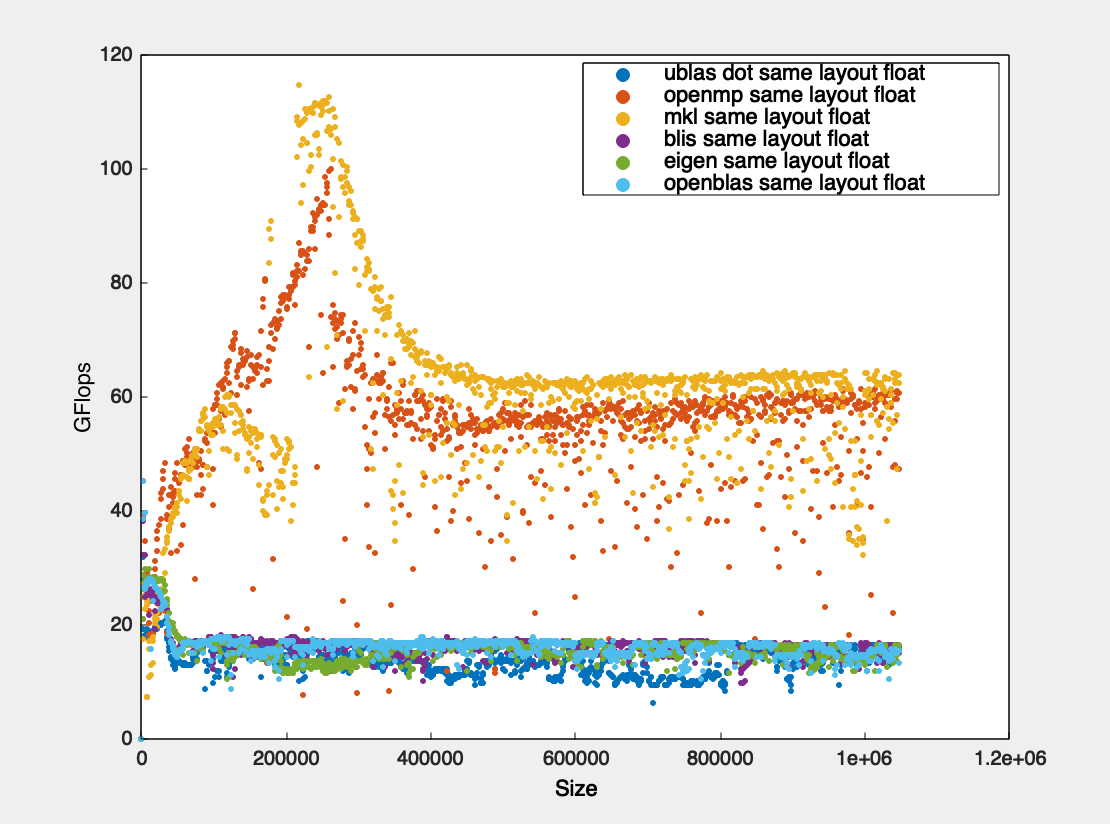
\includegraphics[width=8cm]{../assets/mtm/float_GflopsVsSize.png} }}%
    \label{fig:mtm_col_Sgflop220}
    \qquad
    \subfloat[\centering Double-Precision]{{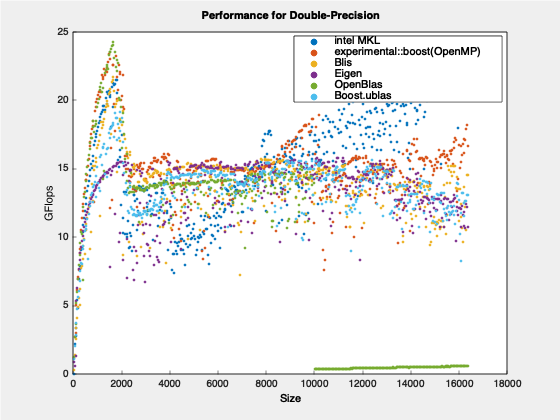
\includegraphics[width=8cm]{../assets/mtm/double_GflopsVsSize.png} }}%
    \label{fig:mtm_col_Dgflop220}
\end{figure}

\begin{figure}[htb]
    \centering
    \caption*{Sorted performance measurements of ?gemm implementations}
    \subfloat[\centering Single-Precision]{{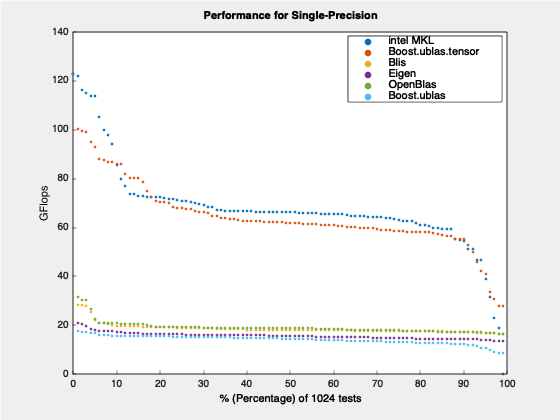
\includegraphics[width=8cm]{../assets/mtm/float_GflopsVsSize_per.png} }}%
    \label{fig:mtm_col_Sgflop_per220}
    \qquad
    \subfloat[\centering Double-Precision]{{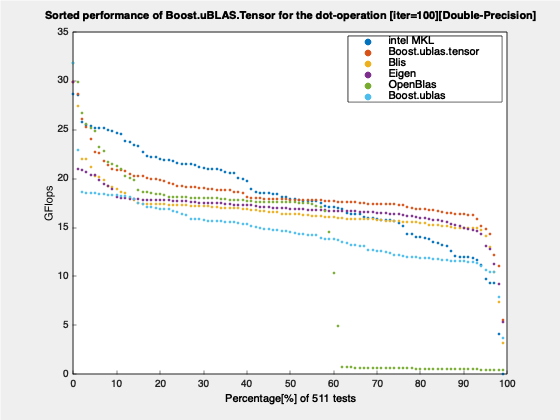
\includegraphics[width=8cm]{../assets/mtm/double_GflopsVsSize_per.png} }}%
    \label{fig:mtm_col_Dgflop_per220}
\end{figure}

\begin{figure}[htb]
    \centering
    \caption*{Comparison of the Boost.uBLAS.Tensor ?gemm implementation}
    \subfloat[\centering Single-Precision]{{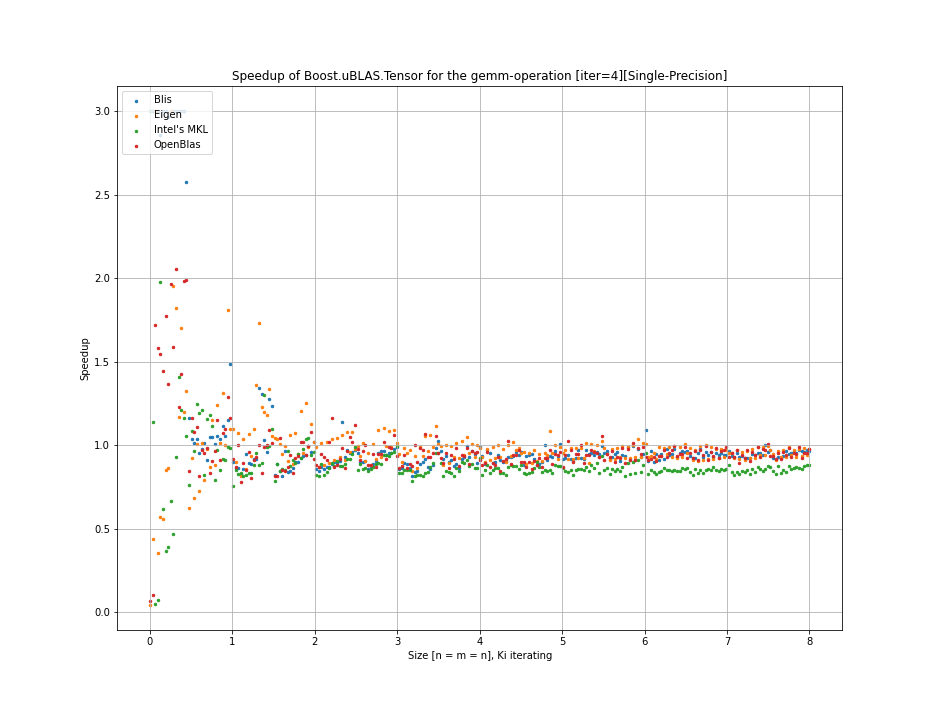
\includegraphics[width=8cm]{../assets/mtm/float_Speedup.png} }}%
    \label{fig:mtm_col_Sspeedup220}
    \qquad
    \subfloat[\centering Double-Precision]{{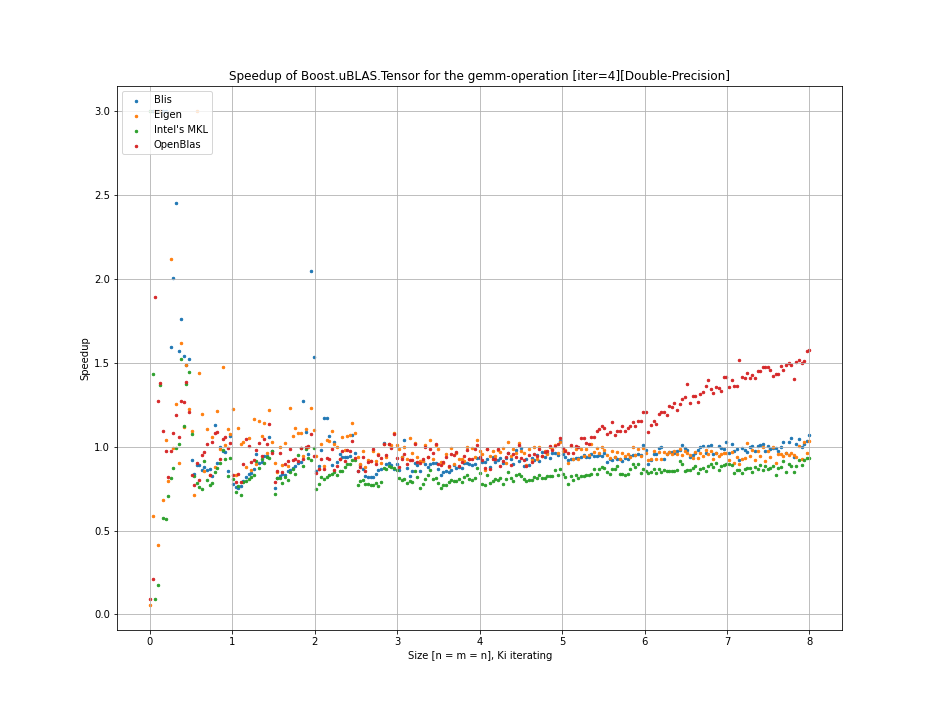
\includegraphics[width=8cm]{../assets/mtm/double_Speedup.png} }}%
    \label{fig:mtm_col_Dspeedup220}
\end{figure}

\begin{figure}[htb]
    \centering
    \caption*{Comparison of the Boost.uBLAS.Tensor ?gemm implementation [sorted]}
    \subfloat[\centering Single-Precision]{{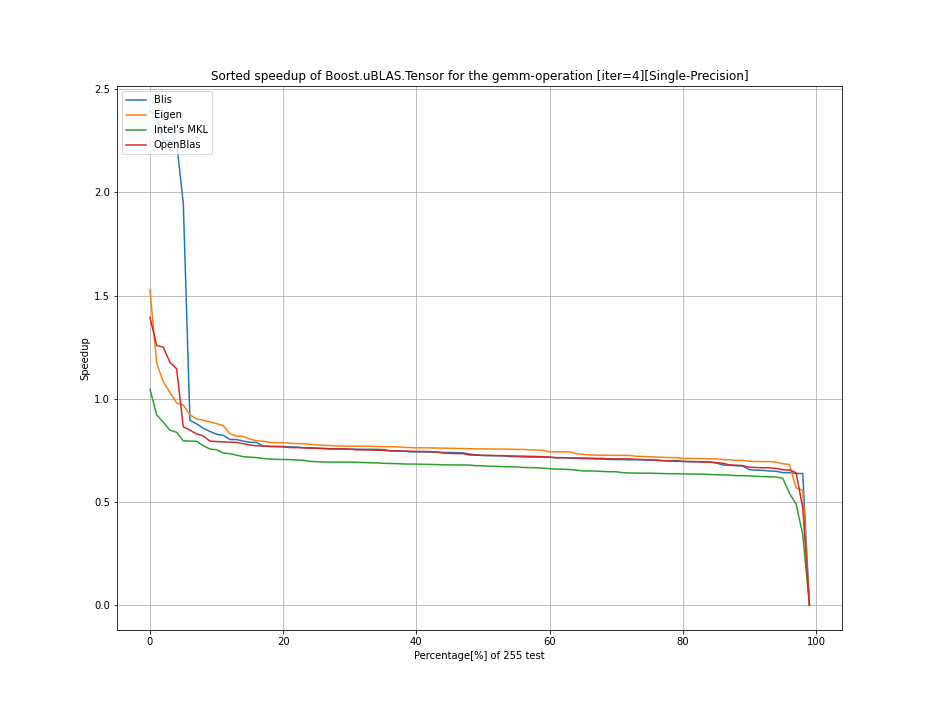
\includegraphics[width=8cm]{../assets/mtm/float_Speedup_per.png} }}%
    \label{fig:mtm_col_Sspeedup_per220}
    \qquad
    \subfloat[\centering Double-Precision]{{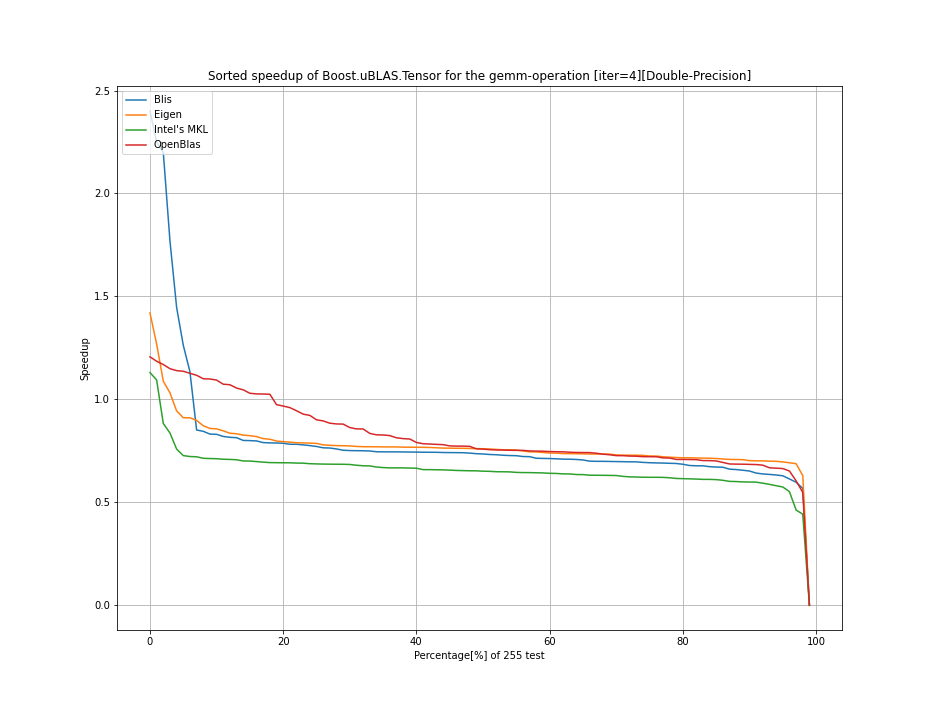
\includegraphics[width=8cm]{../assets/mtm/double_Speedup_per.png} }}%
    \label{fig:mtm_col_Dspeedup_per220}
\end{figure}

\begin{table}[ht]
    \centering
    \caption{Speedup Summary For Single-Precision}
    \begin{tabular}{|l|c|c|}
        \hline
        \textbf{Implementation} & \textbf{Speedup $\geq$ 1 [\%]} & \textbf{Speedup $\geq$ 2 [\%]}\\
        \hline
        OpenBLAS    & $4$ & $0$ \\
        \hline
        Eigen       & $2$ & $0$ \\
        \hline
        Blis        & $5$ & $3$ \\
        \hline
        Intel's MKL & $0$ & $0$ \\
        \hline
    \end{tabular}
    
    \begin{tabular}{|l|c|c|}
        \hline
        \textbf{Implementation} & \textbf{Speed-down $\geq$ 1 [\%]} & \textbf{Speed-down $\geq$ 2 [\%]}\\
        \hline
        OpenBLAS    & $99$ & $99$ \\
        \hline
        Eigen       & $99$ & $99$ \\
        \hline
        Blis        & $99$ & $99$ \\
        \hline
        Intel's MKL & $99$ & $99$ \\
        \hline
    \end{tabular}
    
    \vspace*{1 cm}

    \centering
    \caption{Speedup Summary For Double-Precision}
    \begin{tabular}{|l|c|c|}
        \hline
        \textbf{Implementation} & \textbf{Speedup $\geq$ 1 [\%]} & \textbf{Speedup $\geq$ 2 [\%]}\\
        \hline
        OpenBLAS    & $18$ & $0$ \\
        \hline
        Eigen       & $3$ & $0$ \\
        \hline
        Blis        & $6$ & $2$ \\
        \hline
        Intel's MKL & $2$ & $0$ \\
        \hline
    \end{tabular}
    
    \begin{tabular}{|l|c|c|}
        \hline
        \textbf{Implementation} & \textbf{Speed-down $\geq$ 1 [\%]} & \textbf{Speed-down $\geq$ 2 [\%]}\\
        \hline
        OpenBLAS    & $99$ & $99$ \\
        \hline
        Eigen       & $99$ & $99$ \\
        \hline
        Blis        & $99$ & $99$ \\
        \hline
        Intel's MKL & $99$ & $99$ \\
        \hline
    \end{tabular}
\end{table}

